\section{Experiments}
\label{sec:experiments}

We propose a novel sketch-to-face translation model which is robust to hand-drawn sketches. We conduct extensive experiments to demonstrate the effectiveness of our model in generating high quality realistic face image from sketches. 

\paragraph{Implementation Details}
We implement our model on Pytorch~\cite{Pytorch}. Both generators share an encoder-residual-decoder structure except that an SAP is added to the front of the . The encoder contains four downsample convolutional layers, while the decoder contains four upsample convolutional layers. Nine residual blocks are added between the encoder and decoder to enlarge the capacity of generator. Weights of residual blocks and decoders of two generators share with each other. The multi-scale discriminator consists of three sub-networks for three scales separately. Each sub-network contains four downsample convolutional layers. Instance normalization~\cite{IN} is applied after convolutional layers to stabilize training. ReLU~\cite{ReLU} is used as activation for generators and LeakyReLU~\cite{LeakyReLU} for discriminator. 
%

\paragraph{Training Details}
All the networks are trained by Adam optimizer~\cite{Adam} with $\beta_1=0.5$ and $\beta_2=0.999$. The initial learning rate is set to $0.0002$ for each training stage and starts decay at the half of each stage. Batch size is 32. The entire training schedule takes about three days on four NVIDIA GTX 1080Ti GPUs with 11GB GPU memory.

\paragraph{Data}
CelebA-HQ~\cite{PGGAN} is a large-scale face image dataset which contains 30K $1024\times1024$ high-resolution face images. We use face images in this dataset as real images.
CelebAMask-HQ~\cite{CelebAMask-HQ} offers manually-annotated face semantic masks for CelebA-HQ with 19 classes including all facial components and accessories such as skin, nose, eyes, eyebrows, ears, mouth, lip, hair, hat, eyeglass, earring, necklace, neck, and cloth. We utilize semantic masks in this dataset to extract semantic boundary maps as edge-aligned sketches. Both real images and sketches are resized to $256\times256$ in our experiments.

\paragraph{Baseline Model} 
Pix2pixHD~\cite{pix2pixHD} is a state-of-the-art image-to-image translation model for high-resolution images. 
With the edge-aligned sketches and face real images, we train pix2pixHD with its low-resolution version of generator ('global generator') as a baseline model in our experiment, denoted as \textit{baseline}. 
In order to conduct a fair comparison on generalization, we also train the baseline model with both edge-aligned sketches and deformed sketches, denoted as \textit{baseline\_deform}.

\subsection{Evaluation Metrics} 
Evaluating the performance of generative models has been studied in image generation literature.
It is proven to be a complicated task because a model with good performance with respect to one criterion does not necessarily imply good performance with respect to another criterion~\cite{GANs_equal}. 
A proper evaluation metrics should be able to present the joint statistics between conditional input samples and generated images which means traditional metrics, such as pixel-wise mean-squared error, do not reveal the performance of generative models. 
Therefore, we utilize three popular quantitative perceptual evaluation metrics based on deep neural features: Inception Score (IS)~\cite{Improved_Techniques}, Fréchet Inception Distance (FID)~\cite{FID},
and Kernel Inception Distance (KID)~\cite{KID}. 
These metrics are proven to be consistent with human evaluation in assessing the realism of images.

\paragraph{Inception Score (IS)}
IS applies an Inception model pre-trained on ImageNet to extract features of generated images and computes the KL divergence between the conditional class distribution and the marginal class distribution. We note that IS is reported to biased in some cases because its evaluation is based more on the recognizability rather than on the realism of the generated samples~\cite{evaluation}. Higher IS presents higher quality of generative images.

\paragraph{Fréchet Inception Distance (FID)}
FID is a recently proposed evaluation metrics for generative models and proven to be consistent with human evaluation in assessing the realism of images. FID computes Wasserstein-2 distance between features of generated images and real images which are also extracted by a pre-trained Inception model. Lower FID indicates that the generative distribution is closer to the real distribution.

\paragraph{Kernel Inception Distance (KID)}
KID measures the distance of two distributions by calculating the squared maximum mean discrepancy between Inception features. KID is pointed out to an unbiased estimator with a cubic kernel~\cite{KID}. Models with better performance are supposed to achieve a lower KID.

\subsection{Generative Quality Comparison with Image Translation networks}

Existing image-to-image translation models can be trained for sketch-to-face translation using the paired dataset. 
Since the quality of the generated images presents the basic performance of a generative model, we first compare the generative quality between our model and existing models using three evaluation metrics of IS, FID, and KID. In this experiment, existing models are trained by edge-aligned face sketches and the corresponding real face images. 
We test both our model and existing models with edge-aligned sketches in the test set. Two more existing methods are included in this experiments besides the baseline model. Pix2pix~\cite{pix2pix} is the first general image-to-image translation framework which is able to applied to a variety of applications by switching the training data. We use the default setting to train pix2pix model with paired edge-aligned sketches and real face images. Lines2face~\cite{Lines2Face} is proposed as a sketch-to-face translation model which aims to preserve the entire facial structure by introducing self-attention mechanism to image-to-image translation framework. Lines2face is original trained with edge maps. We only switch the training data to paired edge-aligned sketches and real face images, leaving other settings unchanged.

Table~\ref{tab:generative_quality} shows the quantitative results of this experiment. \td{The our model surpasses all existing models with respect to all three evaluation metrics and xxxxxxxxxx.}

Visual results are shown in Figure~\ref{fig:generative_quality}

\begin{table}[h]
	\centering	
	\caption{Results of generative quality comparison.}
	\begin{tabular}{|c|c|c|c|c|}\hline
		& Pix2pix \cite{pix2pix} & Baseline~\cite{pix2pixHD} & Baseline\_deform & Ours \\\hline
		IS & $2.186$ & $2.298$ & $2.369$ & $2.411$\\\hline
		FID & $289.3$ & 259.1$ & $625.98$ & $\textbf{606.73}$\\\hline
		KID & $-$ & $-$ & $-$ & $-$\\\hline
	\end{tabular}
	\label{tab:generative_quality}
\end{table} 

\begin{figure}
	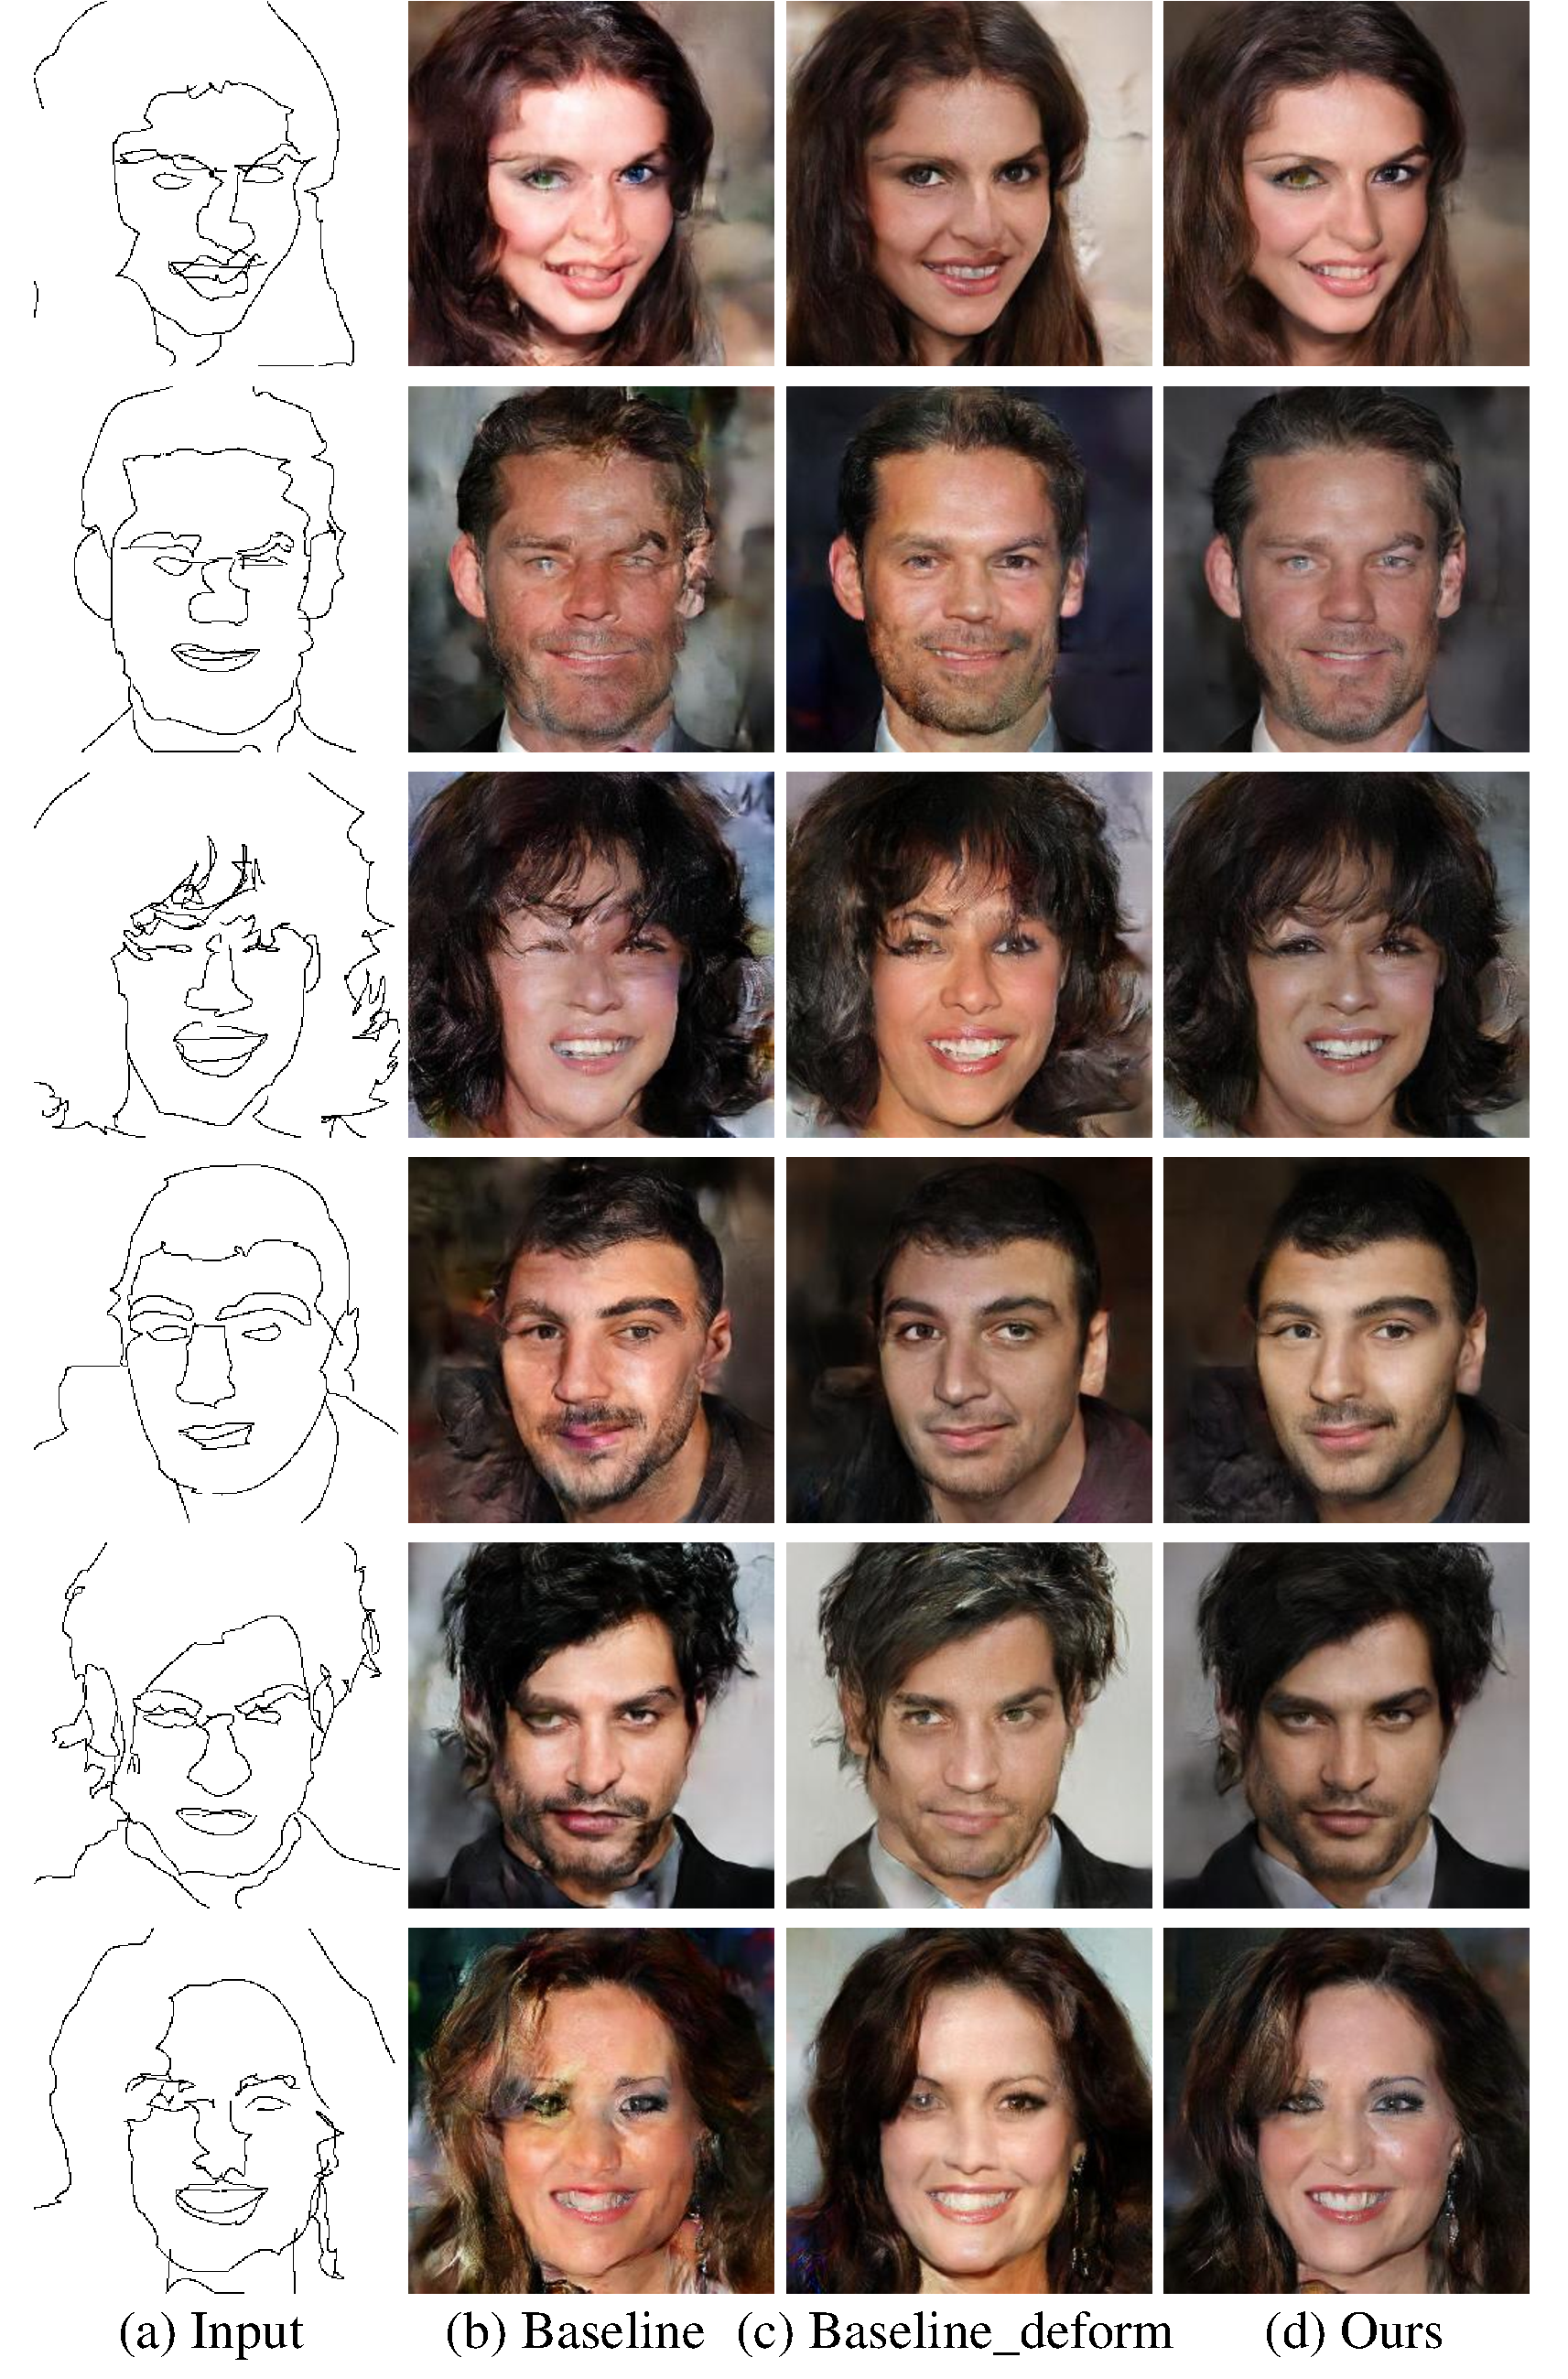
\includegraphics[width=0.9\linewidth]{figs/generalization_examples}
	\caption{\td{Result analyze, use generalization\_examples.pdf as placeholder}}
	\label{fig:generative_quality}
\end{figure}

\subsection{Generalization Comparison with Baseline Model}

In order to verify the generalization ability of our model, we design several experiments and compare our model with the baseline model by testing with sketches of different levels of deformation, well-drawn sketches and poor-drawn sketches.

\subsubsection{Different Levels of Deformation}
As mentioned in Subsection~\ref{subsec:algorithm_data}, we deform a edge-aligned sketch $S$ to obtain a corresponding deformed sketch $S'$ by vectorizing strokes in $S$ and adding random offsets to the control points and end points of the vectorized strokes. The maximum offset $d$ is set to $11$ in the training data. We further create more deformed sketches with different levels of deformation, denoted as $S_d'$, by modifying the maximum offset $d$, where $d$ indicates the level of deformation. We examine the generalization ability of our model and baseline model on these sketches. Note that the \textit{baseline} is trained with only edge-aligned sketches while our model and \textit{baseline\_deform} model are trained both edge-aligned sketches and deformed sketches with $d=11$.

In this experiment, the input sketches are deformed by large offsets where the maximum $d$ is set to $30$. 
As shown in Figure~\ref{fig:generalization_examples}, strokes in the largely deformed sketches are quite different from those in the training sketches including edge-aligned sketches $S$ and deformed sketches $S_11'$. \td{xxxxx}.
\begin{figure}
	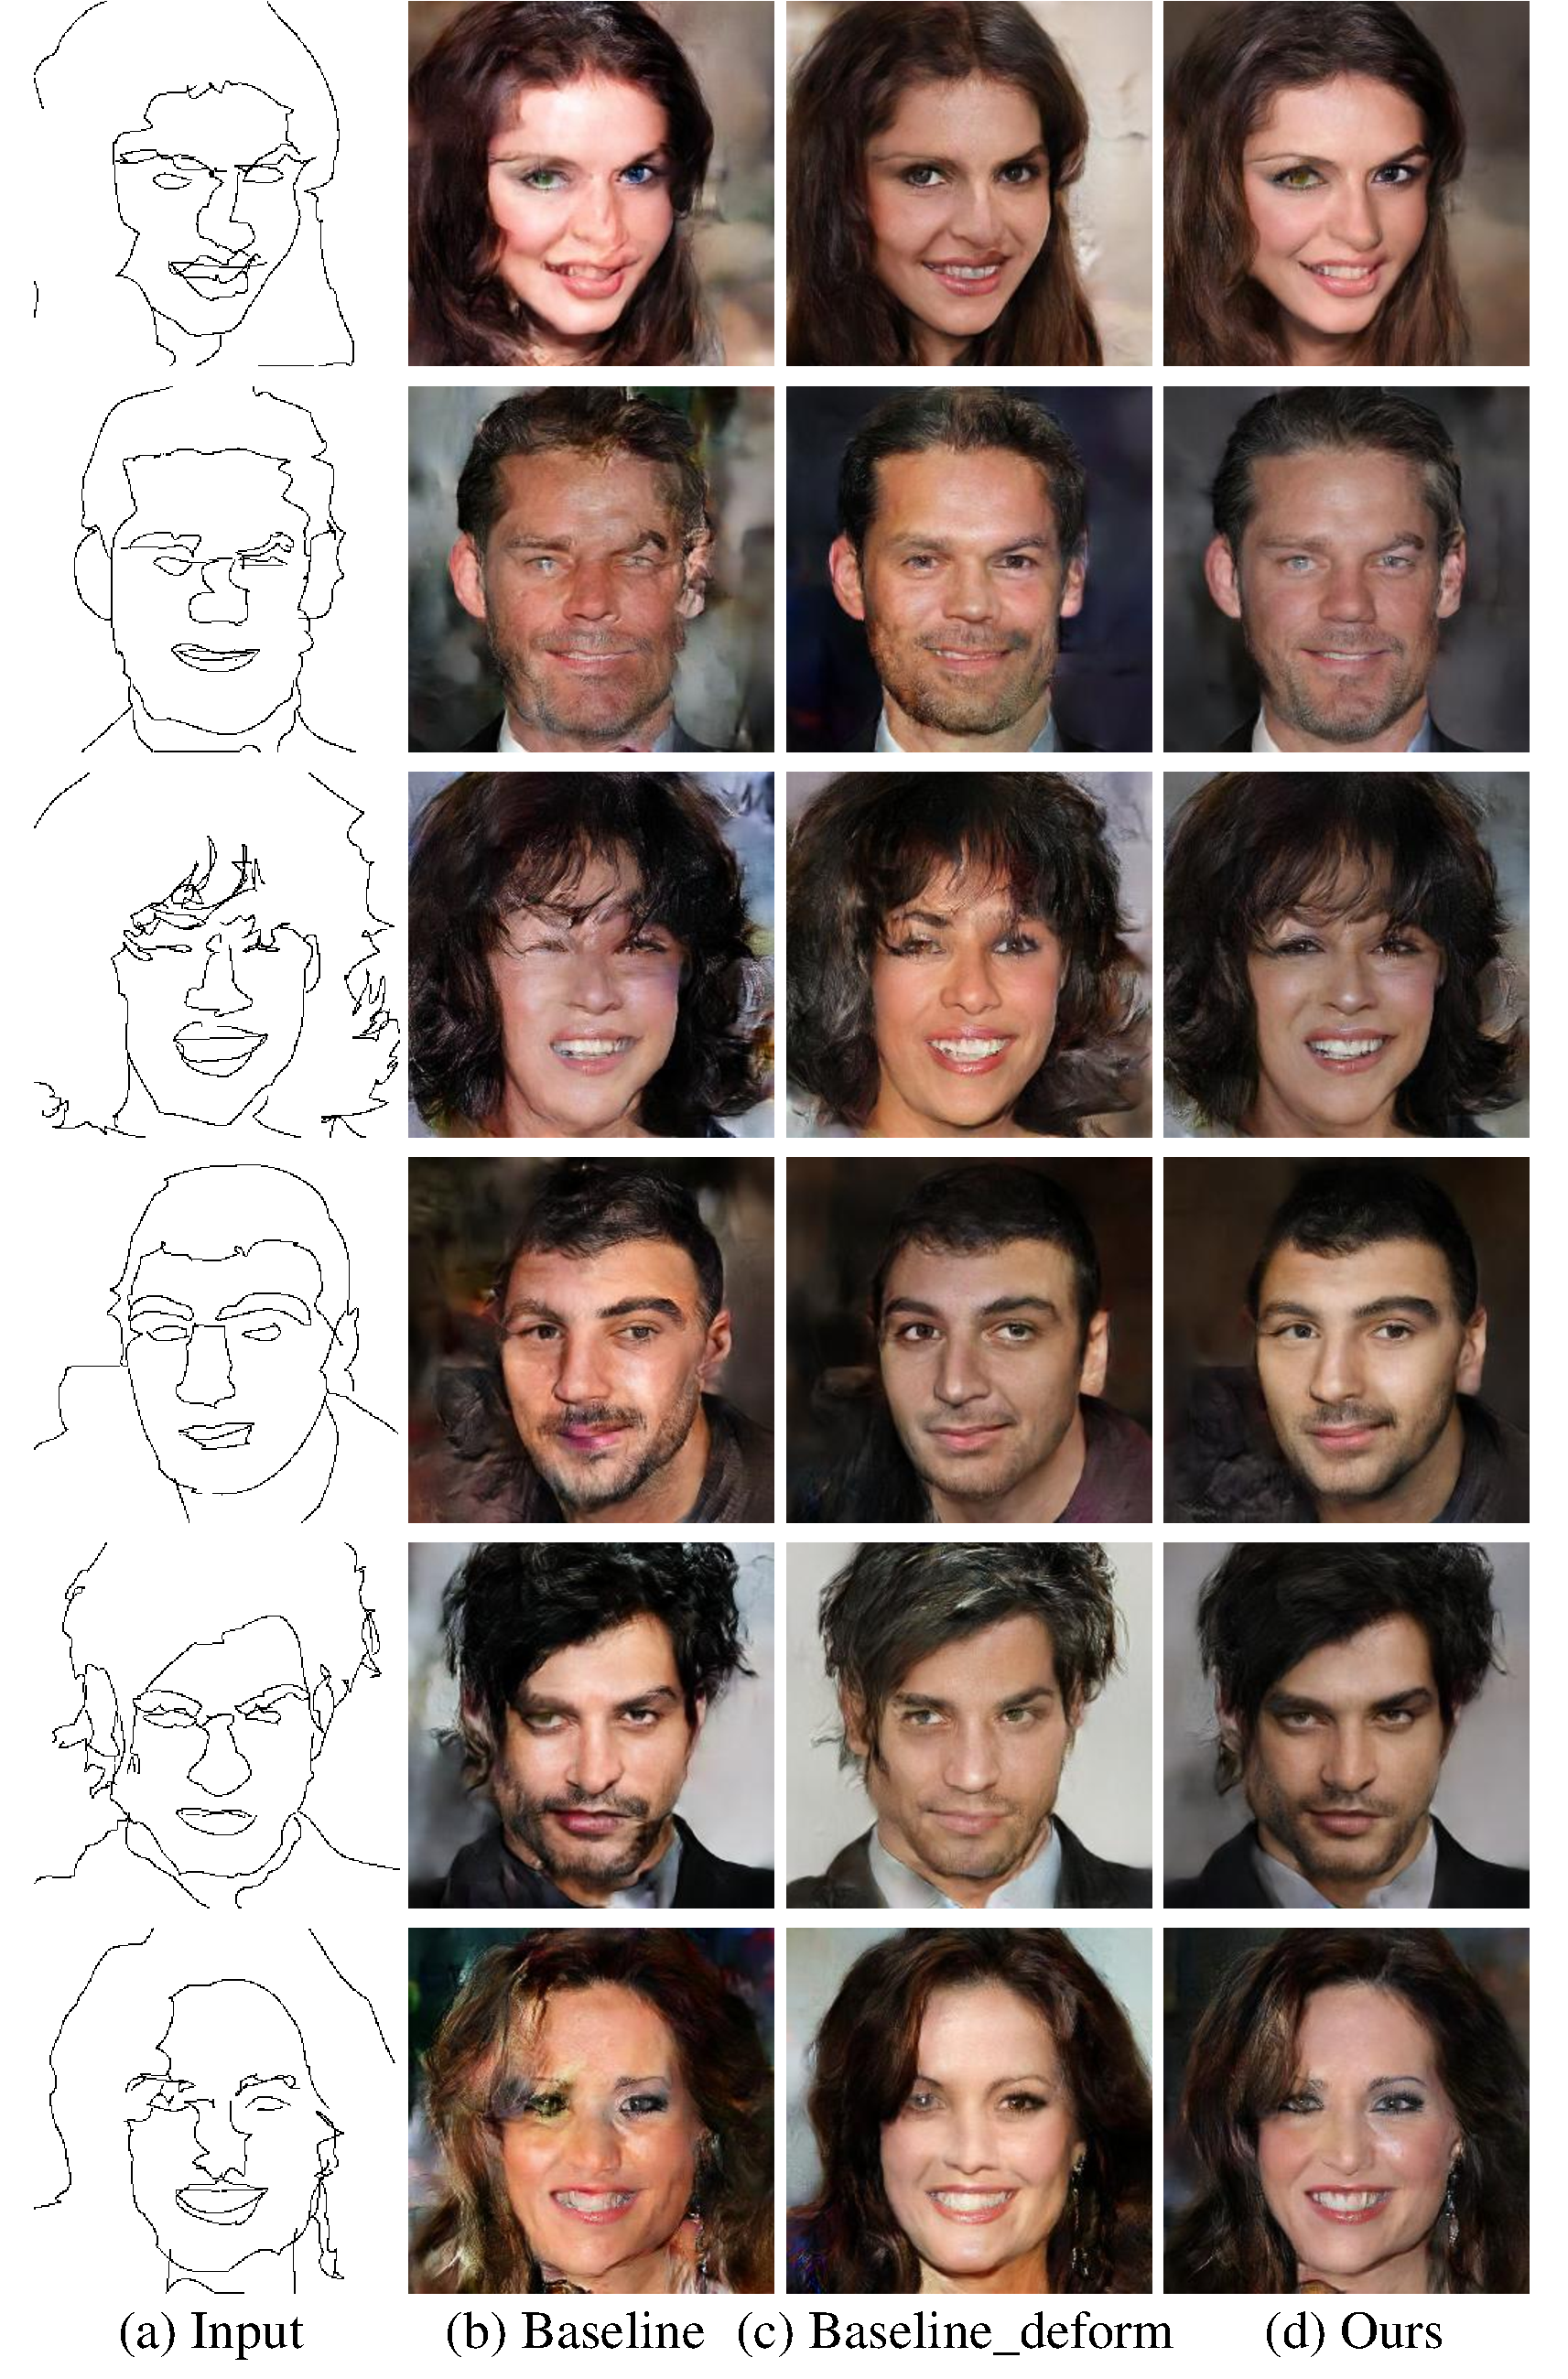
\includegraphics[width=0.9\linewidth]{figs/generalization_examples}
	\caption{\td{Result analyze}}
	\label{fig:generalization_examples}
\end{figure}

\subsubsection{Hand-Drawn Sketches}
In this experiment, we examine model generalization ability by comparing performances of our model with baseline model tested with two kinds of hand-drawn sketches: expert hand-drawn sketches and common hand-drawn sketches.

\paragraph{Expert Sketches}
We invite professional users with well-trained drawing skills to draw expert sketches for testing. These expert sketches are drawn on a drawing board device which enables strokes to be drawn smoothly and accurately. Figure~\ref{fig:expert_sketches} shows that texture of our results are more realistic and those of both \textit{baseline} model and \textit{baseline\_deform} model are blurred in some facial areas. 

\begin{figure}
	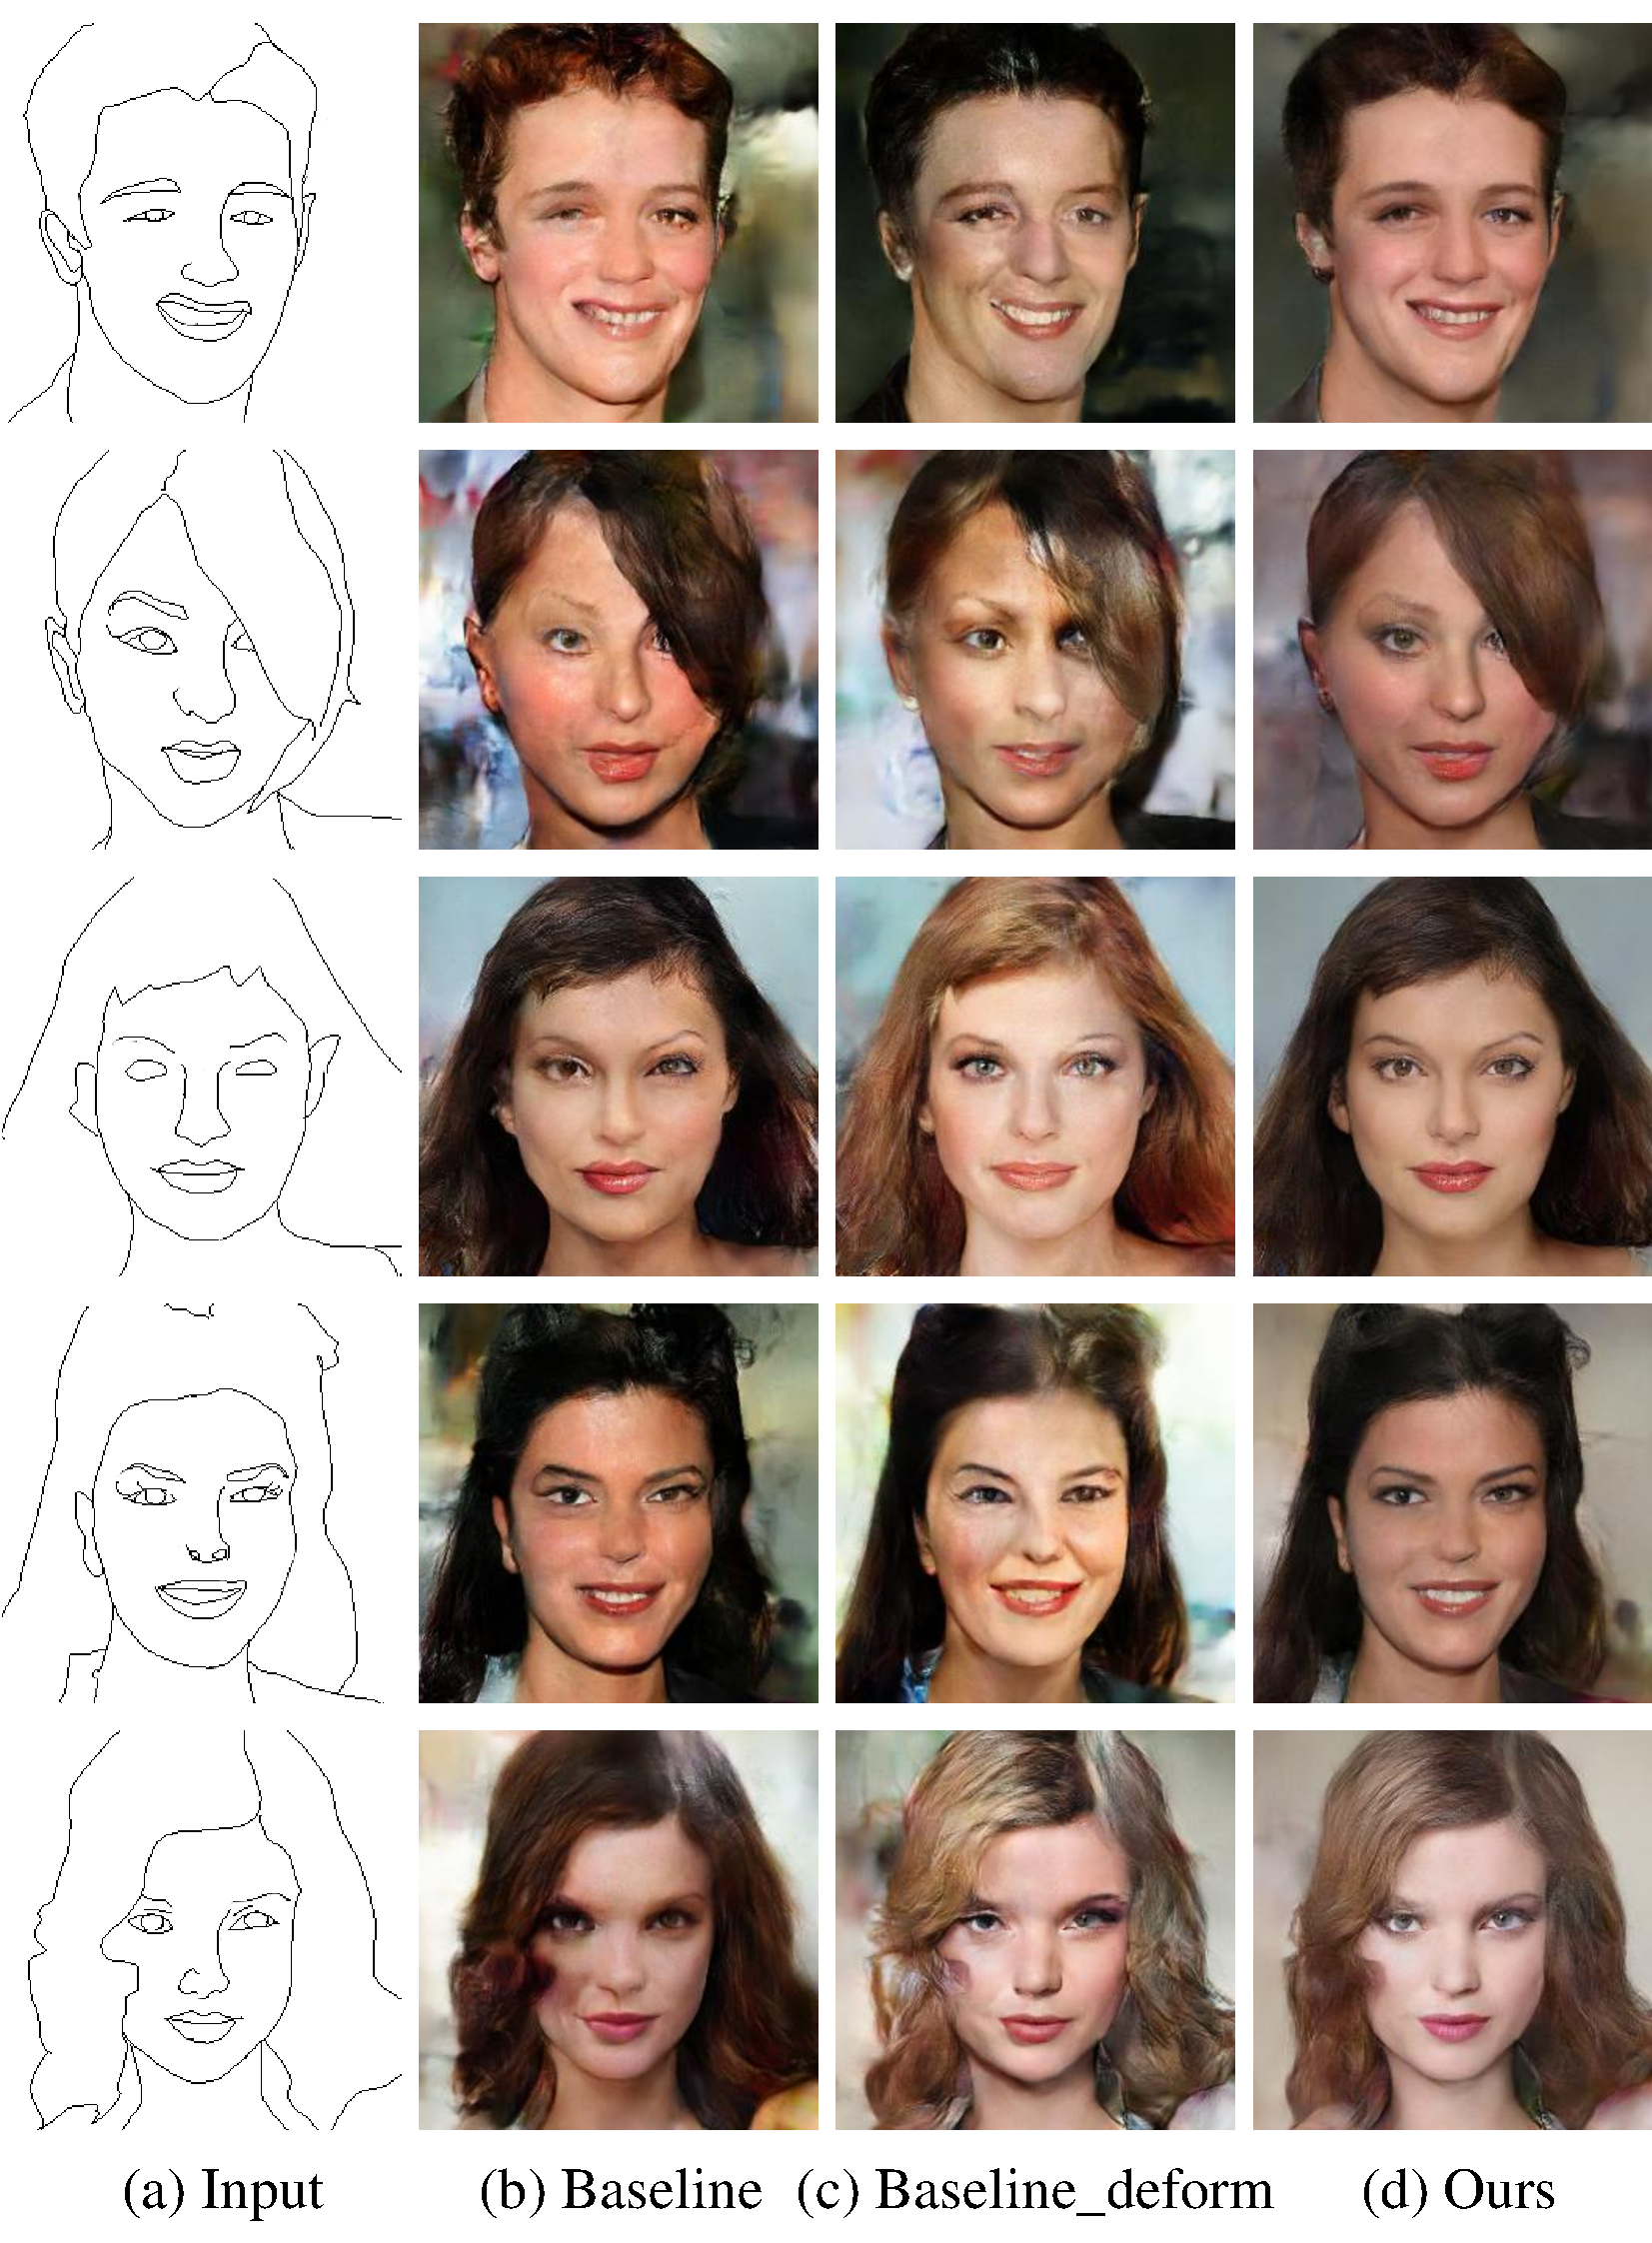
\includegraphics[width=0.9\linewidth]{figs/expertsketches}
	\caption{\td{Result analyze}}
	\label{fig:expert_sketches}
\end{figure}


\paragraph{Common Sketches}
We also introduce common user without drawing skills to draw common hand-drawn sketches. The common sketches are drawn by common users using a mouse of computer. Hence, strokes of the common sketches depicts the ideal face images roughly. Also, common sketches turn to be of different levels of details. For example, some sketches contains several strokes inside the hair areas which are blanket in training sketches. Results shown in Figure~\ref{fig:common_sketches} demonstrate that our model is robust to these common sketches while the different stroke styles and different detail levels damage the quality of results from \textit{baseline} model and \textit{baseline\_deform} model heavily.


\begin{figure}
	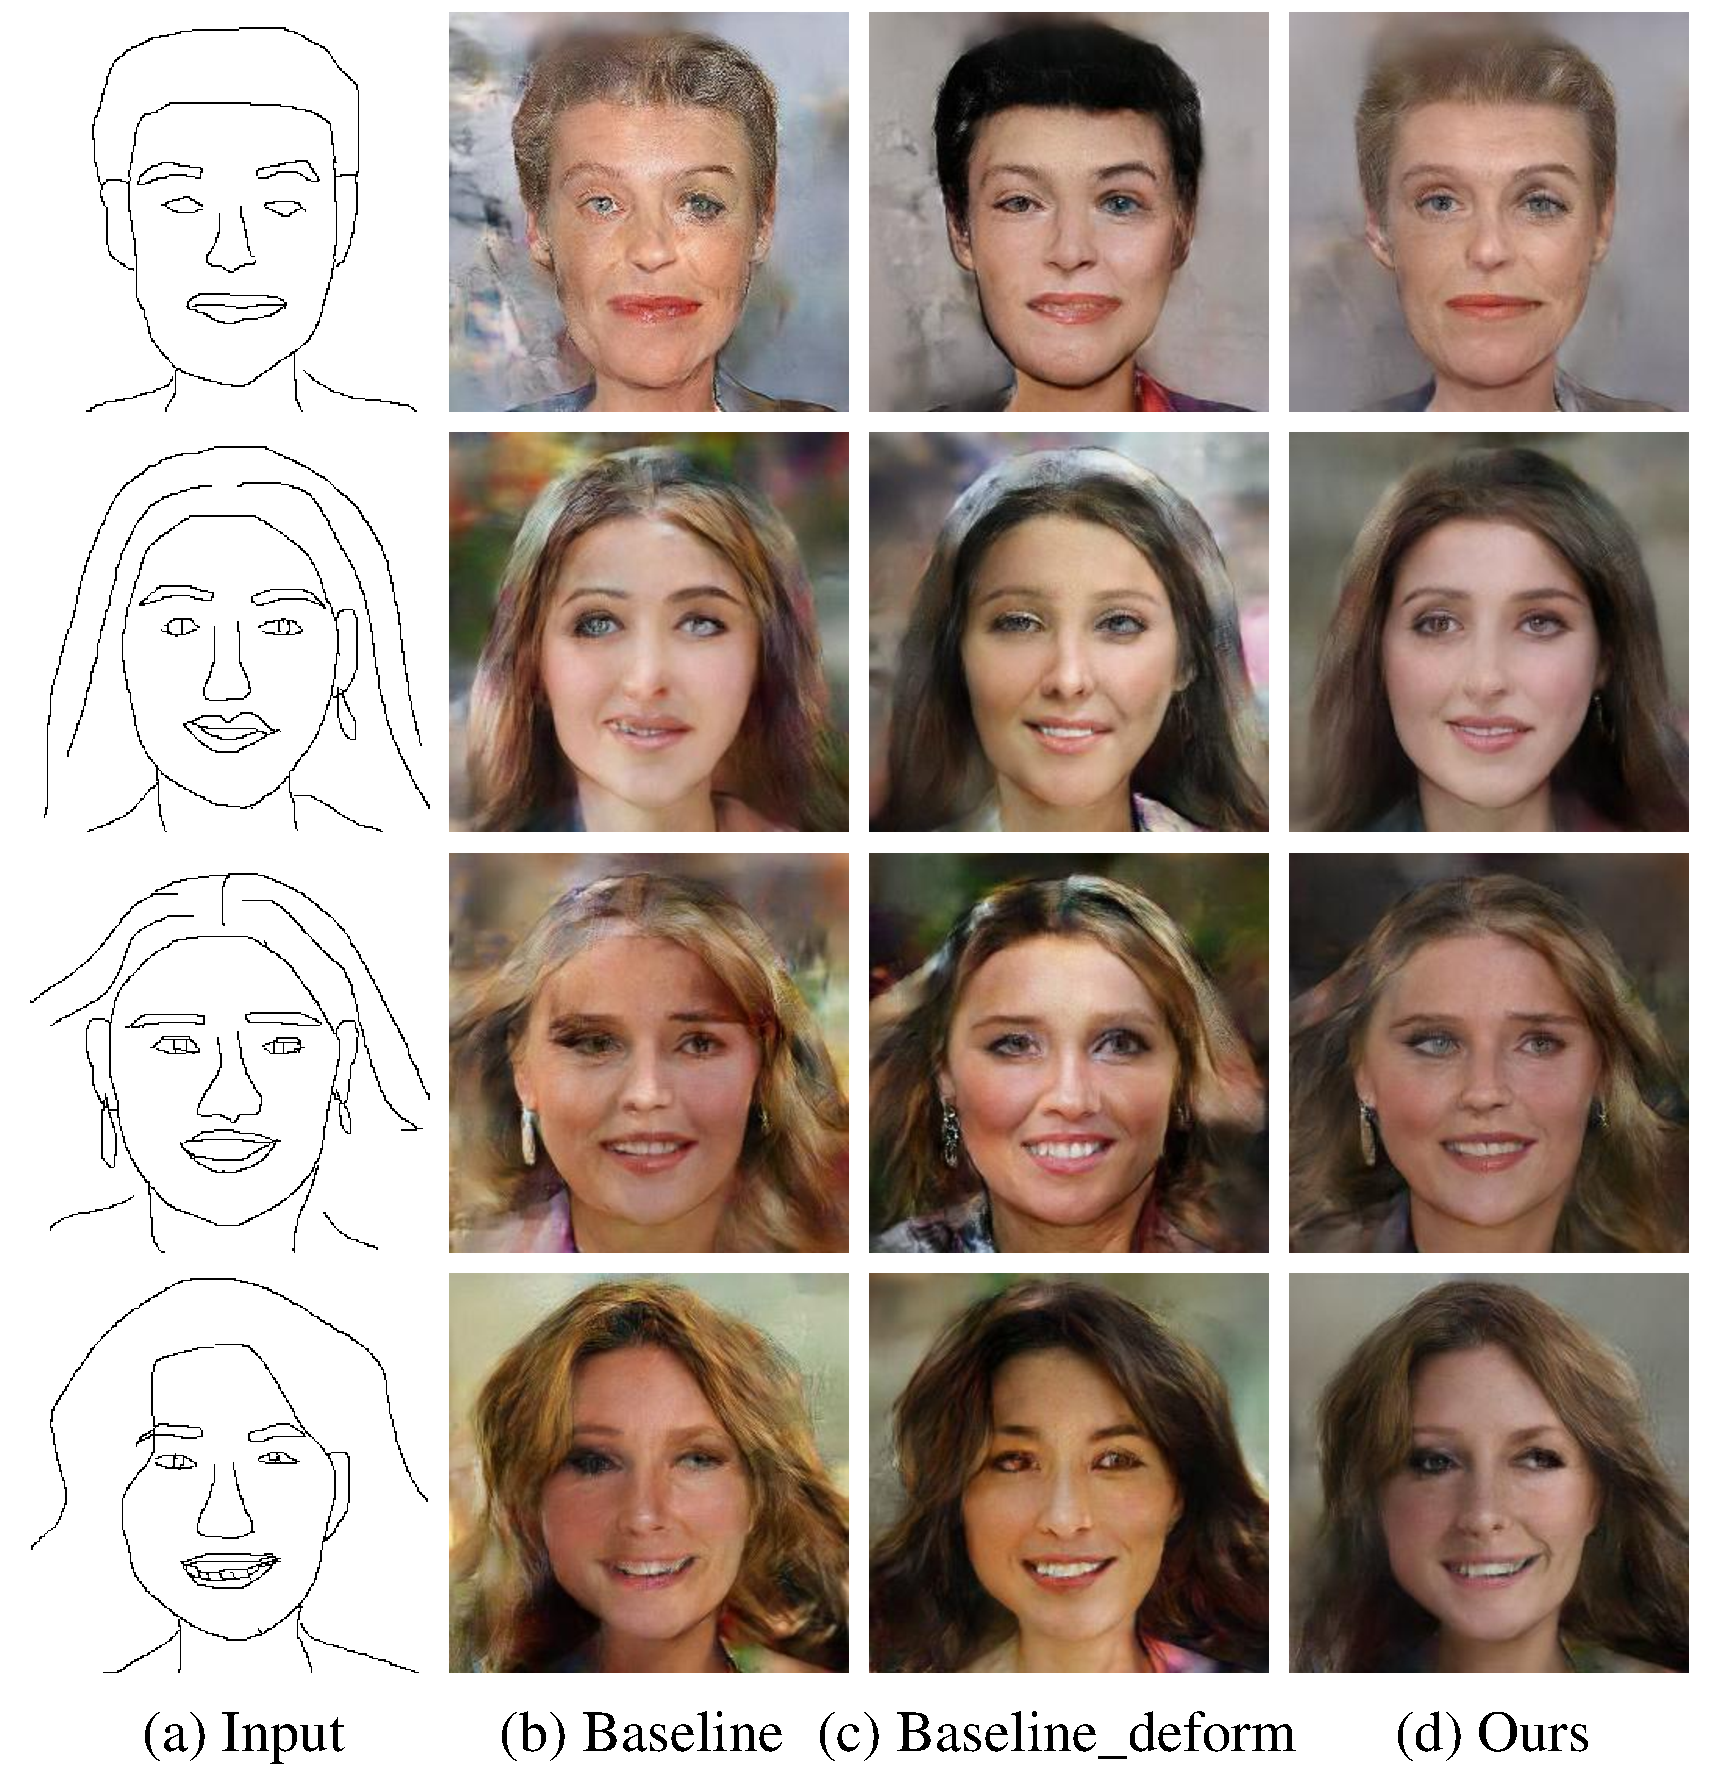
\includegraphics[width=0.9\linewidth]{figs/commonsketches}
	\caption{\td{Result analyze}}
	\label{fig:common_sketches}
\end{figure}


\subsection{Limitations and future work}

\